\documentclass{beamer}
\usepackage[utf8]{inputenc}
\usepackage[T1]{fontenc}
\usepackage{fancyvrb}
\title{Deep Learning on the IMDB Dataset}
\date{WASP Deep Learning}
\author[Agents 47]{The Hitmen --- Agents 47}

%\usepackage{enumitem}

\usepackage{pgfplots}
\pgfplotsset{compat=1.8}
\usepackage{pgfplotstable}
\usepgfplotslibrary{groupplots}

\newlength\figureheight
\newlength\figurewidth

\usetheme{wasp}

\graphicspath{{./graphics/}}

\usepackage{lipsum}
\newcommand\blfootnote[1]{%
	\begingroup
	\renewcommand\thefootnote{}\footnote{#1}%
	\addtocounter{footnote}{-1}%
	\endgroup
}

\begin{document}

\begin{frame}
  \titlepage
\end{frame}


\begin{frame}{Convnets}{Convolutional Neural Networks}

  \begin{itemize}

  \item[Training] Using all data, we reached the best result after around 1 or 2
    epochs to around 93.5 \%. By using less, say 20 \% of the data, training
    improved for up to 4 epochs, but the validation results were considerably
    worse (73 \%). Note however that training with less data is considerably
    faster.

  \item[Batch] Smaller batches train slightly faster, but doesn't otherwise
    affect validation results much (Got 94.1 \% with batch size 64). Too big
    batches may however consume too much memory for efficient training.

  \item[Reviews/Unique] Increasing these values can add a significant amount of
    data to the model, and thus \textbf{might} improve the result (93.7 \%), but
    will also take longer to train. Reducing it barely changs the result. (93.1
    \%).

  \item[Dropout] 20\% dropout helps slightly: 94.7 \%.  40\% dropout helps a bit
    more: 95.5 \%. Even higher (80 \%) didn't improve the final result, but did
    make the learning process improve for all 10 epochs.

  \item[Architecture] Krohn's architecture seems to perform slightly better, but
    takes a little longer to train than Chollet's. Comparing this with a network
    architecture with only dense layers (~88 \%), convolutional architectures seem
    superior.

  \item[Smaller Network]

  \end{itemize}

\end{frame}


\begin{frame}{Convnets}{Training History}

  \begin{columns}
    \begin{column}{0.5\textwidth}
      \begin{figure}[ht]
        \centering
        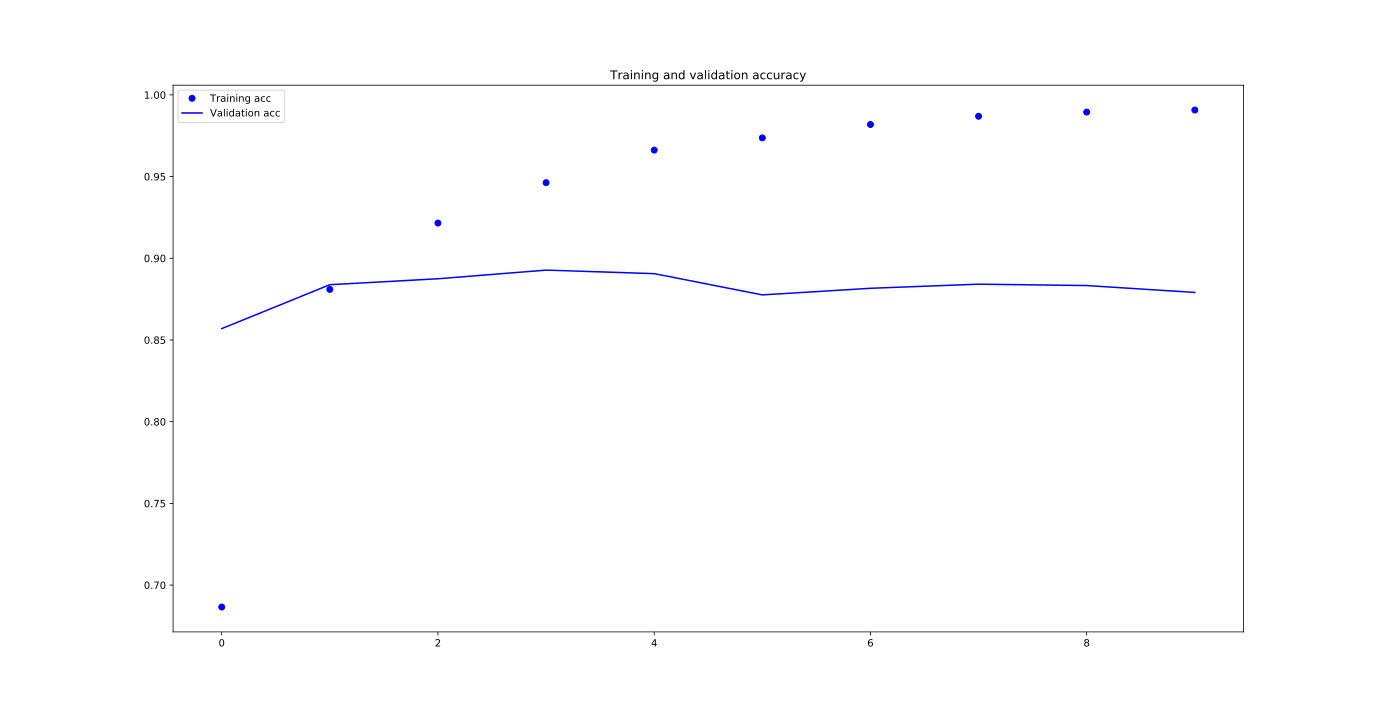
\includegraphics[width=1.2\textwidth]{convnet_training}
      \end{figure}

    \end{column}
    \begin{column}{0.5\textwidth}
      \begin{figure}[ht]
        \centering
        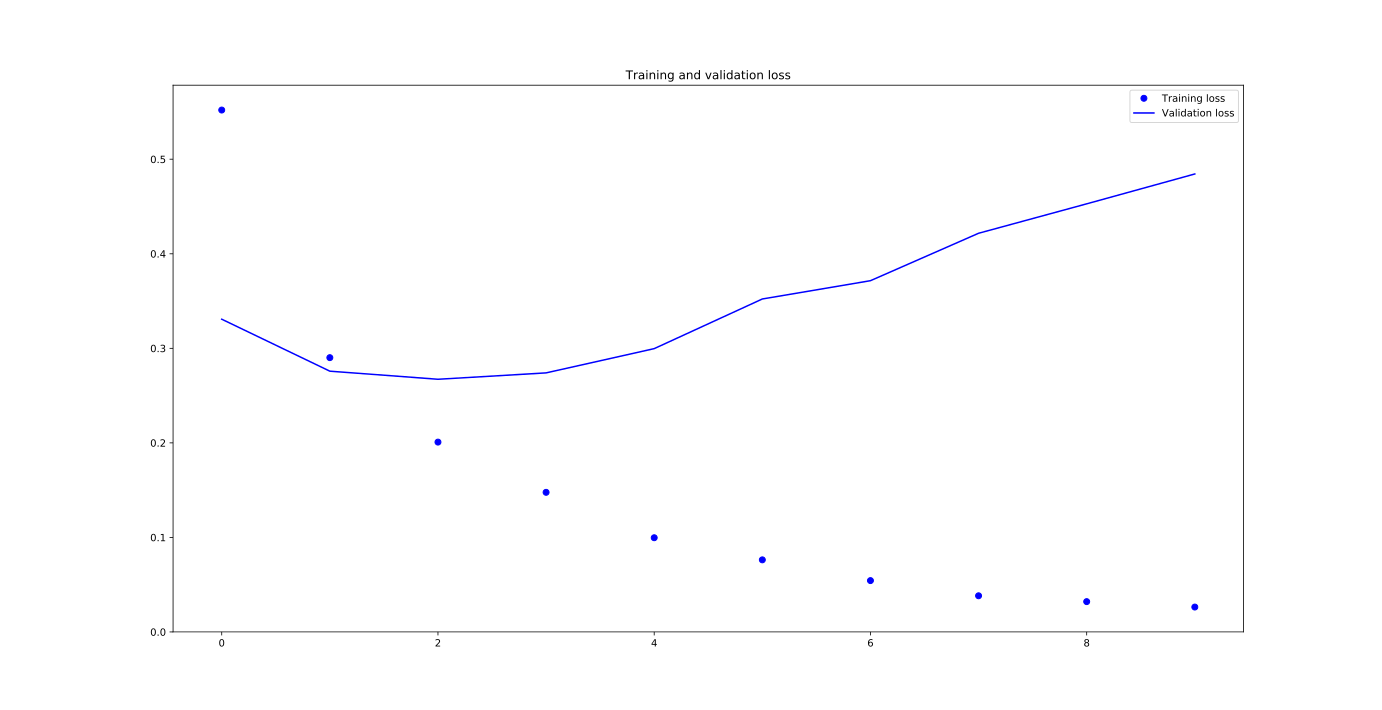
\includegraphics[width=1.2\textwidth]{convnet_loss}
      \end{figure}

    \end{column}
  \end{columns}

\end{frame}


\begin{frame}{Convnets}{Classification Confidence}

  \begin{figure}[ht]
    \centering
    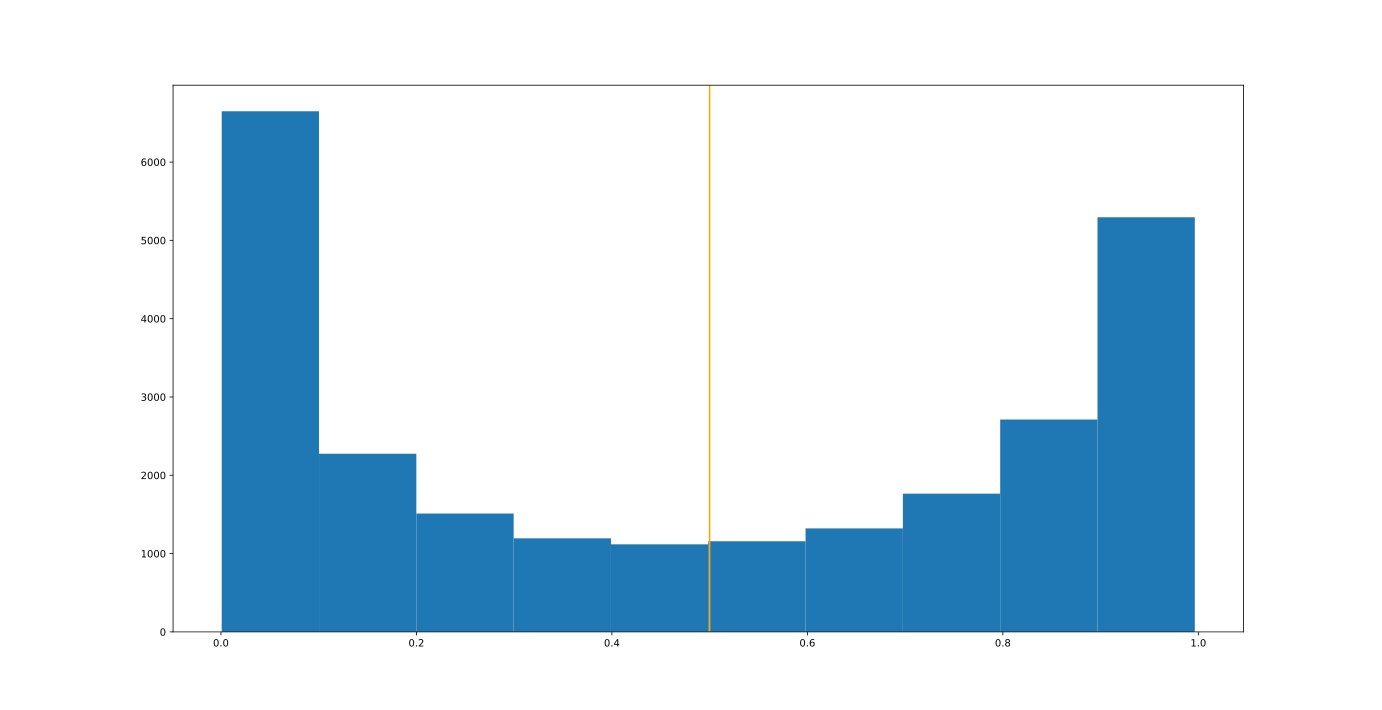
\includegraphics[width=0.7\textwidth]{convnet_histogram}
  \end{figure}

\end{frame}

\begin{frame}{Convnets}{Why Convolutions for NLP?}

  \begin{itemize}

  \item Intuitively, a 1D convolution would look both forwards and backwards in
    a sentence, mimicking how the natural language refers to earlier or coming
    words.

  \item Training for more than 2 or 3 epochs doesn't appear to be beneficial for
    classification of this data. This does however depend quite a lot on
    hyper-parameter choices.

  \item Best validation score: 95.96 \%.

  \end{itemize}

\end{frame}



\begin{frame}{RNN}{Recurrent Neural Networks}

	Output of the layer is fed back into the layer, which can be seen as a recursion over a time series.

	\begin{figure}
		\centering
		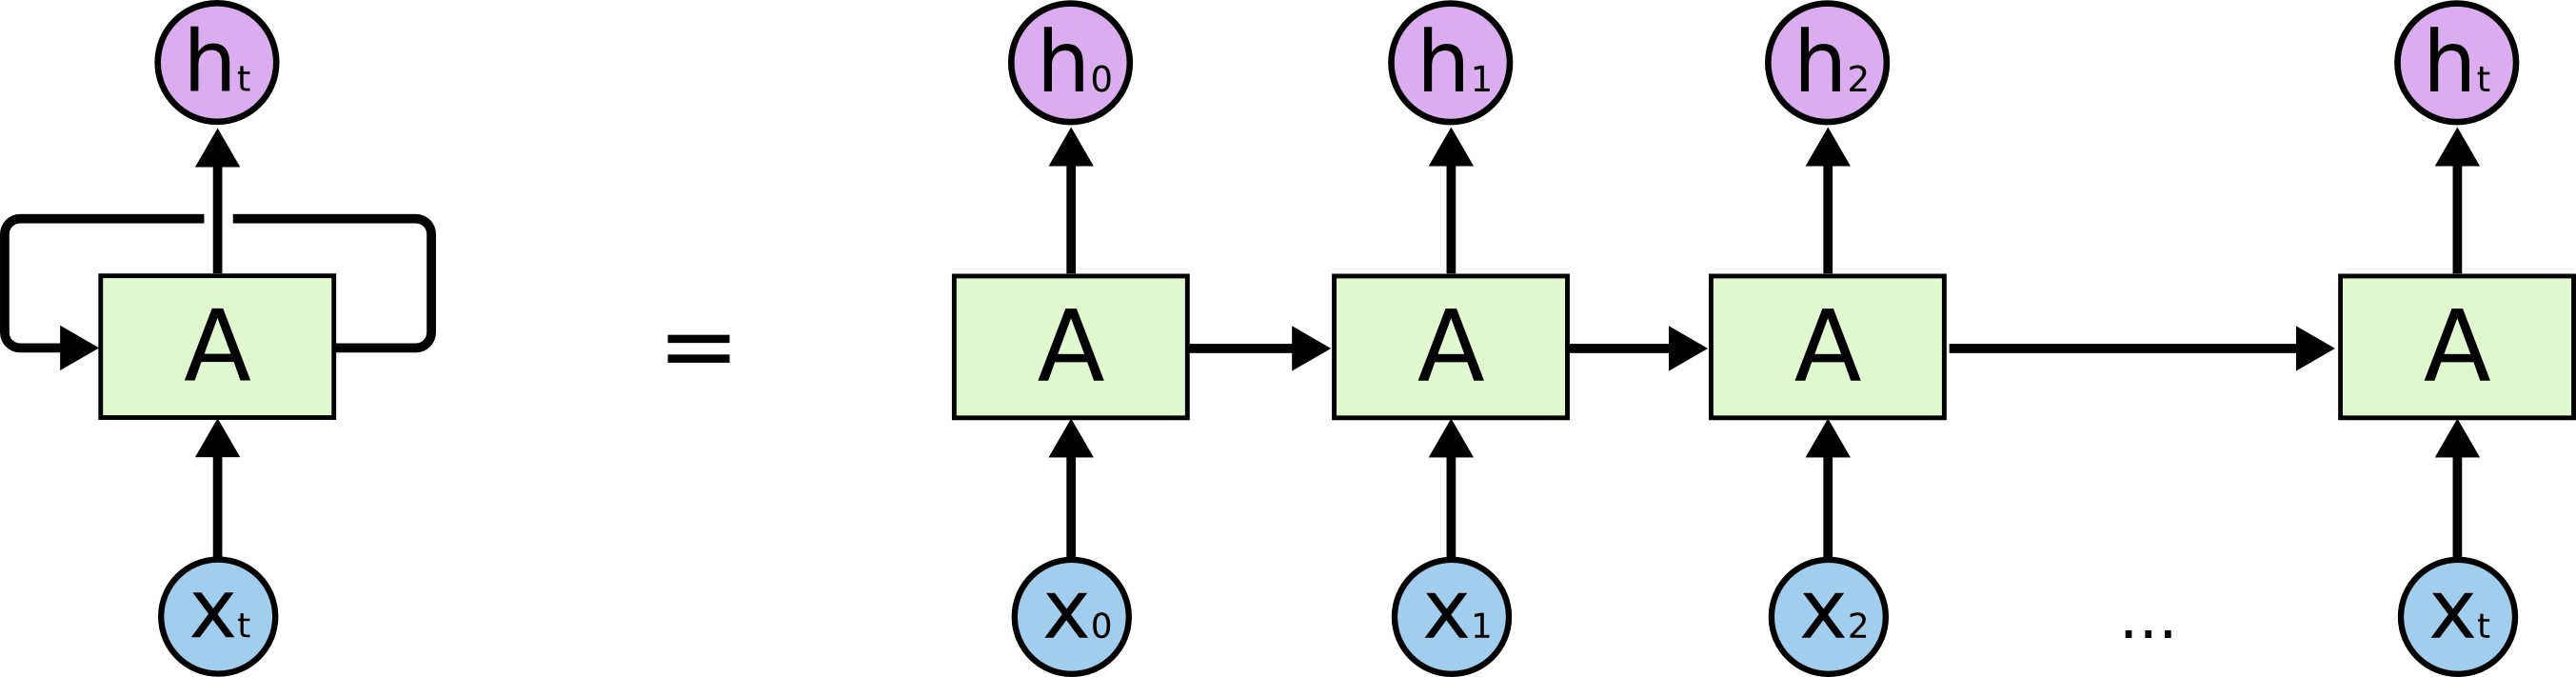
\includegraphics[width=0.7\linewidth]{graphics/RNN-unrolled.png}
	\end{figure}

	Testing the impact of stacking layers, 4 models in total are trained. Model 1 contains 1 32-sized RNN layer with 0.2 dropout, Model 2 contains 2 such layers and so on. This is then trained for 5 epochs with 128 batch size. 


\blfootnote{\tiny Image courtesy of Christopher Olah, \url{http://colah.github.io/posts/2015-08-Understanding-LSTMs/}}
  
\end{frame}

\begin{frame}{RNN}{Recurrent Neural Networks}
	\begin{figure}
	\centering

	\setlength\figureheight{3cm}
	\setlength\figurewidth{0.5\linewidth}
	
	% This file was created by matplotlib2tikz v0.6.18.
\begin{tikzpicture}

\begin{groupplot}[group style={group size=2 by 2}]
\nextgroupplot[
height=\figureheight,
tick align=outside,
tick pos=left,
title={Model 1},
width=\figurewidth,
x grid style={lightgray!92.02614379084967!black},
xmin=-0.2, xmax=4.2,
y grid style={lightgray!92.02614379084967!black},
ymin=0.5, ymax=1,
xticklabels={,,,,}
]
\addplot [semithick, blue, mark=*, mark size=3, mark options={solid}, only marks, forget plot]
table [row sep=\\]{%
0	0.605879999961853 \\
1	0.775800000038147 \\
2	0.865720000019073 \\
3	0.912959999980926 \\
4	0.939960000019074 \\
};
\addplot [semithick, blue, forget plot]
table [row sep=\\]{%
0	0.762640000038147 \\
1	0.773159999980927 \\
2	0.842439999980927 \\
3	0.828439999961853 \\
4	0.852039999980926 \\
};
\nextgroupplot[
height=\figureheight,
tick align=outside,
tick pos=left,
title={Model 2},
width=\figurewidth,
x grid style={lightgray!92.02614379084967!black},
xmin=-0.2, xmax=4.2,
y grid style={lightgray!92.02614379084967!black},
ymin=0.5, ymax=1,
xticklabels={,,,,}
]
\addplot [semithick, blue, mark=*, mark size=3, mark options={solid}, only marks, forget plot]
table [row sep=\\]{%
0	0.587199999961853 \\
1	0.854319999961853 \\
2	0.872839999961853 \\
3	0.912079999980926 \\
4	0.942880000019073 \\
};
\addplot [semithick, blue, forget plot]
table [row sep=\\]{%
0	0.81604 \\
1	0.8648 \\
2	0.844160000038147 \\
3	0.849200000019073 \\
4	0.849999999961853 \\
};
\nextgroupplot[
height=\figureheight,
tick align=outside,
tick pos=left,
title={Model 3},
width=\figurewidth,
x grid style={lightgray!92.02614379084967!black},
xmin=-0.2, xmax=4.2,
y grid style={lightgray!92.02614379084967!black},
ymin=0.5, ymax=1
]
\addplot [semithick, blue, mark=*, mark size=3, mark options={solid}, only marks, forget plot]
table [row sep=\\]{%
0	0.522080000019074 \\
1	0.773879999961853 \\
2	0.882079999961853 \\
3	0.926399999961853 \\
4	0.956040000019074 \\
};
\addplot [semithick, blue, forget plot]
table [row sep=\\]{%
0	0.582559999961853 \\
1	0.821520000019073 \\
2	0.816400000019074 \\
3	0.81756 \\
4	0.840599999980926 \\
};
\nextgroupplot[
height=\figureheight,
tick align=outside,
tick pos=left,
title={Model 4},
width=\figurewidth,
x grid style={lightgray!92.02614379084967!black},
xmin=-0.2, xmax=4.2,
y grid style={lightgray!92.02614379084967!black},
ymin=0.5, ymax=1
]
\addplot [semithick, blue, mark=*, mark size=3, mark options={solid}, only marks, forget plot]
table [row sep=\\]{%
0	0.498879999980927 \\
1	0.50836 \\
2	0.601960000019073 \\
3	0.791760000019074 \\
4	0.869559999961853 \\
};
\addplot [semithick, blue, forget plot]
table [row sep=\\]{%
0	0.499999999980927 \\
1	0.525439999990463 \\
2	0.770719999961853 \\
3	0.824199999961853 \\
4	0.820239999961853 \\
};
\end{groupplot}

\end{tikzpicture}
	\caption{Training (circle) vs Validation (line) accuracy.} 
	\end{figure}
\end{frame}

\begin{frame}{RNN}{Recurrent Neural Networks}
	
	\noindent
	\begin{minipage}{0.45\textwidth}%
		 The different models obtain a ROC value of 
		 \begin{itemize}%[noitemsep,topsep=0pt,parsep=0pt,partopsep=0pt]
		 	\item Model 1: 86.34
		 	\item Model 2: 93.49
		 	\item Model 3: 66.09
		 	\item Model 4: 52.38
		 \end{itemize}
	 	Considering the histograms as well, it can be concluded that adding additional layers \emph{can} improve performace but also increases the risk of not converging as seen in Model 3 and 4.
	\end{minipage} \hfill
	\begin{minipage}{0.45\textwidth}%
		\begin{figure}
			\centering
			
			\setlength\figureheight{3cm}
			\setlength\figurewidth{0.5\linewidth}
			
			% This file was created by matplotlib2tikz v0.6.18.
\begin{tikzpicture}

\definecolor{color1}{rgb}{1,0.647058823529412,0}
\definecolor{color0}{rgb}{0.12156862745098,0.466666666666667,0.705882352941177}

\begin{groupplot}[group style={group size=2 by 2}]
\nextgroupplot[
height=\figureheight,
tick align=outside,
tick pos=left,
title={Model 1},
width=\figurewidth,
x grid style={lightgray!92.02614379084967!black},
xmin=0, xmax=1,
y grid style={lightgray!92.02614379084967!black},
ymin=0, ymax=596.4,
xticklabels={,,,,}
]
\draw[fill=color0,draw opacity=0] (axis cs:0.0138896042481065,0) rectangle (axis cs:0.0236279208492488,56);
\draw[fill=color0,draw opacity=0] (axis cs:0.0236279208492488,0) rectangle (axis cs:0.0333662374503911,147);
\draw[fill=color0,draw opacity=0] (axis cs:0.0333662374503911,0) rectangle (axis cs:0.0431045540515333,181);
\draw[fill=color0,draw opacity=0] (axis cs:0.0431045540515333,0) rectangle (axis cs:0.0528428706526756,276);
\draw[fill=color0,draw opacity=0] (axis cs:0.0528428706526756,0) rectangle (axis cs:0.0625811872538179,346);
\draw[fill=color0,draw opacity=0] (axis cs:0.0625811872538179,0) rectangle (axis cs:0.0723195038549602,385);
\draw[fill=color0,draw opacity=0] (axis cs:0.0723195038549602,0) rectangle (axis cs:0.0820578204561025,384);
\draw[fill=color0,draw opacity=0] (axis cs:0.0820578204561025,0) rectangle (axis cs:0.0917961370572448,386);
\draw[fill=color0,draw opacity=0] (axis cs:0.0917961370572448,0) rectangle (axis cs:0.101534453658387,382);
\draw[fill=color0,draw opacity=0] (axis cs:0.101534453658387,0) rectangle (axis cs:0.111272770259529,418);
\draw[fill=color0,draw opacity=0] (axis cs:0.111272770259529,0) rectangle (axis cs:0.121011086860672,460);
\draw[fill=color0,draw opacity=0] (axis cs:0.121011086860672,0) rectangle (axis cs:0.130749403461814,470);
\draw[fill=color0,draw opacity=0] (axis cs:0.130749403461814,0) rectangle (axis cs:0.140487720062956,522);
\draw[fill=color0,draw opacity=0] (axis cs:0.140487720062956,0) rectangle (axis cs:0.150226036664098,531);
\draw[fill=color0,draw opacity=0] (axis cs:0.150226036664099,0) rectangle (axis cs:0.159964353265241,542);
\draw[fill=color0,draw opacity=0] (axis cs:0.159964353265241,0) rectangle (axis cs:0.169702669866383,568);
\draw[fill=color0,draw opacity=0] (axis cs:0.169702669866383,0) rectangle (axis cs:0.179440986467525,563);
\draw[fill=color0,draw opacity=0] (axis cs:0.179440986467525,0) rectangle (axis cs:0.189179303068668,530);
\draw[fill=color0,draw opacity=0] (axis cs:0.189179303068668,0) rectangle (axis cs:0.19891761966981,498);
\draw[fill=color0,draw opacity=0] (axis cs:0.19891761966981,0) rectangle (axis cs:0.208655936270952,439);
\draw[fill=color0,draw opacity=0] (axis cs:0.208655936270952,0) rectangle (axis cs:0.218394252872094,469);
\draw[fill=color0,draw opacity=0] (axis cs:0.218394252872095,0) rectangle (axis cs:0.228132569473237,483);
\draw[fill=color0,draw opacity=0] (axis cs:0.228132569473237,0) rectangle (axis cs:0.237870886074379,444);
\draw[fill=color0,draw opacity=0] (axis cs:0.237870886074379,0) rectangle (axis cs:0.247609202675521,374);
\draw[fill=color0,draw opacity=0] (axis cs:0.247609202675521,0) rectangle (axis cs:0.257347519276664,368);
\draw[fill=color0,draw opacity=0] (axis cs:0.257347519276664,0) rectangle (axis cs:0.267085835877806,341);
\draw[fill=color0,draw opacity=0] (axis cs:0.267085835877806,0) rectangle (axis cs:0.276824152478948,353);
\draw[fill=color0,draw opacity=0] (axis cs:0.276824152478948,0) rectangle (axis cs:0.286562469080091,322);
\draw[fill=color0,draw opacity=0] (axis cs:0.286562469080091,0) rectangle (axis cs:0.296300785681233,334);
\draw[fill=color0,draw opacity=0] (axis cs:0.296300785681233,0) rectangle (axis cs:0.306039102282375,308);
\draw[fill=color0,draw opacity=0] (axis cs:0.306039102282375,0) rectangle (axis cs:0.315777418883517,300);
\draw[fill=color0,draw opacity=0] (axis cs:0.315777418883517,0) rectangle (axis cs:0.32551573548466,248);
\draw[fill=color0,draw opacity=0] (axis cs:0.32551573548466,0) rectangle (axis cs:0.335254052085802,247);
\draw[fill=color0,draw opacity=0] (axis cs:0.335254052085802,0) rectangle (axis cs:0.344992368686944,263);
\draw[fill=color0,draw opacity=0] (axis cs:0.344992368686944,0) rectangle (axis cs:0.354730685288087,232);
\draw[fill=color0,draw opacity=0] (axis cs:0.354730685288087,0) rectangle (axis cs:0.364469001889229,204);
\draw[fill=color0,draw opacity=0] (axis cs:0.364469001889229,0) rectangle (axis cs:0.374207318490371,216);
\draw[fill=color0,draw opacity=0] (axis cs:0.374207318490371,0) rectangle (axis cs:0.383945635091513,200);
\draw[fill=color0,draw opacity=0] (axis cs:0.383945635091513,0) rectangle (axis cs:0.393683951692656,202);
\draw[fill=color0,draw opacity=0] (axis cs:0.393683951692656,0) rectangle (axis cs:0.403422268293798,226);
\draw[fill=color0,draw opacity=0] (axis cs:0.403422268293798,0) rectangle (axis cs:0.41316058489494,195);
\draw[fill=color0,draw opacity=0] (axis cs:0.41316058489494,0) rectangle (axis cs:0.422898901496083,173);
\draw[fill=color0,draw opacity=0] (axis cs:0.422898901496083,0) rectangle (axis cs:0.432637218097225,169);
\draw[fill=color0,draw opacity=0] (axis cs:0.432637218097225,0) rectangle (axis cs:0.442375534698367,171);
\draw[fill=color0,draw opacity=0] (axis cs:0.442375534698367,0) rectangle (axis cs:0.452113851299509,178);
\draw[fill=color0,draw opacity=0] (axis cs:0.452113851299509,0) rectangle (axis cs:0.461852167900652,170);
\draw[fill=color0,draw opacity=0] (axis cs:0.461852167900652,0) rectangle (axis cs:0.471590484501794,151);
\draw[fill=color0,draw opacity=0] (axis cs:0.471590484501794,0) rectangle (axis cs:0.481328801102936,173);
\draw[fill=color0,draw opacity=0] (axis cs:0.481328801102936,0) rectangle (axis cs:0.491067117704079,149);
\draw[fill=color0,draw opacity=0] (axis cs:0.491067117704079,0) rectangle (axis cs:0.500805434305221,129);
\draw[fill=color0,draw opacity=0] (axis cs:0.500805434305221,0) rectangle (axis cs:0.510543750906363,161);
\draw[fill=color0,draw opacity=0] (axis cs:0.510543750906363,0) rectangle (axis cs:0.520282067507505,154);
\draw[fill=color0,draw opacity=0] (axis cs:0.520282067507505,0) rectangle (axis cs:0.530020384108648,158);
\draw[fill=color0,draw opacity=0] (axis cs:0.530020384108648,0) rectangle (axis cs:0.53975870070979,160);
\draw[fill=color0,draw opacity=0] (axis cs:0.53975870070979,0) rectangle (axis cs:0.549497017310932,144);
\draw[fill=color0,draw opacity=0] (axis cs:0.549497017310932,0) rectangle (axis cs:0.559235333912075,154);
\draw[fill=color0,draw opacity=0] (axis cs:0.559235333912075,0) rectangle (axis cs:0.568973650513217,165);
\draw[fill=color0,draw opacity=0] (axis cs:0.568973650513217,0) rectangle (axis cs:0.578711967114359,144);
\draw[fill=color0,draw opacity=0] (axis cs:0.578711967114359,0) rectangle (axis cs:0.588450283715502,143);
\draw[fill=color0,draw opacity=0] (axis cs:0.588450283715501,0) rectangle (axis cs:0.598188600316644,148);
\draw[fill=color0,draw opacity=0] (axis cs:0.598188600316644,0) rectangle (axis cs:0.607926916917786,150);
\draw[fill=color0,draw opacity=0] (axis cs:0.607926916917786,0) rectangle (axis cs:0.617665233518928,148);
\draw[fill=color0,draw opacity=0] (axis cs:0.617665233518928,0) rectangle (axis cs:0.627403550120071,113);
\draw[fill=color0,draw opacity=0] (axis cs:0.627403550120071,0) rectangle (axis cs:0.637141866721213,158);
\draw[fill=color0,draw opacity=0] (axis cs:0.637141866721213,0) rectangle (axis cs:0.646880183322355,154);
\draw[fill=color0,draw opacity=0] (axis cs:0.646880183322355,0) rectangle (axis cs:0.656618499923497,147);
\draw[fill=color0,draw opacity=0] (axis cs:0.656618499923497,0) rectangle (axis cs:0.66635681652464,155);
\draw[fill=color0,draw opacity=0] (axis cs:0.66635681652464,0) rectangle (axis cs:0.676095133125782,169);
\draw[fill=color0,draw opacity=0] (axis cs:0.676095133125782,0) rectangle (axis cs:0.685833449726924,164);
\draw[fill=color0,draw opacity=0] (axis cs:0.685833449726924,0) rectangle (axis cs:0.695571766328067,166);
\draw[fill=color0,draw opacity=0] (axis cs:0.695571766328067,0) rectangle (axis cs:0.705310082929209,145);
\draw[fill=color0,draw opacity=0] (axis cs:0.705310082929209,0) rectangle (axis cs:0.715048399530351,170);
\draw[fill=color0,draw opacity=0] (axis cs:0.715048399530351,0) rectangle (axis cs:0.724786716131493,212);
\draw[fill=color0,draw opacity=0] (axis cs:0.724786716131493,0) rectangle (axis cs:0.734525032732636,183);
\draw[fill=color0,draw opacity=0] (axis cs:0.734525032732636,0) rectangle (axis cs:0.744263349333778,191);
\draw[fill=color0,draw opacity=0] (axis cs:0.744263349333778,0) rectangle (axis cs:0.75400166593492,179);
\draw[fill=color0,draw opacity=0] (axis cs:0.75400166593492,0) rectangle (axis cs:0.763739982536063,178);
\draw[fill=color0,draw opacity=0] (axis cs:0.763739982536063,0) rectangle (axis cs:0.773478299137205,216);
\draw[fill=color0,draw opacity=0] (axis cs:0.773478299137205,0) rectangle (axis cs:0.783216615738347,223);
\draw[fill=color0,draw opacity=0] (axis cs:0.783216615738347,0) rectangle (axis cs:0.792954932339489,254);
\draw[fill=color0,draw opacity=0] (axis cs:0.79295493233949,0) rectangle (axis cs:0.802693248940632,218);
\draw[fill=color0,draw opacity=0] (axis cs:0.802693248940632,0) rectangle (axis cs:0.812431565541774,226);
\draw[fill=color0,draw opacity=0] (axis cs:0.812431565541774,0) rectangle (axis cs:0.822169882142916,246);
\draw[fill=color0,draw opacity=0] (axis cs:0.822169882142916,0) rectangle (axis cs:0.831908198744059,214);
\draw[fill=color0,draw opacity=0] (axis cs:0.831908198744059,0) rectangle (axis cs:0.841646515345201,254);
\draw[fill=color0,draw opacity=0] (axis cs:0.841646515345201,0) rectangle (axis cs:0.851384831946343,216);
\draw[fill=color0,draw opacity=0] (axis cs:0.851384831946343,0) rectangle (axis cs:0.861123148547486,273);
\draw[fill=color0,draw opacity=0] (axis cs:0.861123148547486,0) rectangle (axis cs:0.870861465148628,255);
\draw[fill=color0,draw opacity=0] (axis cs:0.870861465148628,0) rectangle (axis cs:0.88059978174977,258);
\draw[fill=color0,draw opacity=0] (axis cs:0.88059978174977,0) rectangle (axis cs:0.890338098350912,252);
\draw[fill=color0,draw opacity=0] (axis cs:0.890338098350912,0) rectangle (axis cs:0.900076414952055,248);
\draw[fill=color0,draw opacity=0] (axis cs:0.900076414952055,0) rectangle (axis cs:0.909814731553197,232);
\draw[fill=color0,draw opacity=0] (axis cs:0.909814731553197,0) rectangle (axis cs:0.919553048154339,238);
\draw[fill=color0,draw opacity=0] (axis cs:0.919553048154339,0) rectangle (axis cs:0.929291364755481,235);
\draw[fill=color0,draw opacity=0] (axis cs:0.929291364755481,0) rectangle (axis cs:0.939029681356624,184);
\draw[fill=color0,draw opacity=0] (axis cs:0.939029681356624,0) rectangle (axis cs:0.948767997957766,148);
\draw[fill=color0,draw opacity=0] (axis cs:0.948767997957766,0) rectangle (axis cs:0.958506314558908,138);
\draw[fill=color0,draw opacity=0] (axis cs:0.958506314558908,0) rectangle (axis cs:0.968244631160051,158);
\draw[fill=color0,draw opacity=0] (axis cs:0.968244631160051,0) rectangle (axis cs:0.977982947761193,86);
\draw[fill=color0,draw opacity=0] (axis cs:0.977982947761193,0) rectangle (axis cs:0.987721264362335,39);
\addplot [semithick, color1, forget plot]
table [row sep=\\]{%
0.5	0 \\
0.5	1 \\
};
\nextgroupplot[
height=\figureheight,
tick align=outside,
tick pos=left,
title={Model 2},
width=\figurewidth,
x grid style={lightgray!92.02614379084967!black},
xmin=0, xmax=1,
y grid style={lightgray!92.02614379084967!black},
ymin=0, ymax=1407,
xticklabels={,,,,}
]
\draw[fill=color0,draw opacity=0] (axis cs:0.0144115649163723,0) rectangle (axis cs:0.0241552310064435,147);
\draw[fill=color0,draw opacity=0] (axis cs:0.0241552310064435,0) rectangle (axis cs:0.0338988970965147,745);
\draw[fill=color0,draw opacity=0] (axis cs:0.0338988970965147,0) rectangle (axis cs:0.0436425631865859,1251);
\draw[fill=color0,draw opacity=0] (axis cs:0.0436425631865859,0) rectangle (axis cs:0.0533862292766571,1340);
\draw[fill=color0,draw opacity=0] (axis cs:0.0533862292766571,0) rectangle (axis cs:0.0631298953667283,1206);
\draw[fill=color0,draw opacity=0] (axis cs:0.0631298953667283,0) rectangle (axis cs:0.0728735614567995,1035);
\draw[fill=color0,draw opacity=0] (axis cs:0.0728735614567995,0) rectangle (axis cs:0.0826172275468707,831);
\draw[fill=color0,draw opacity=0] (axis cs:0.0826172275468707,0) rectangle (axis cs:0.0923608936369419,736);
\draw[fill=color0,draw opacity=0] (axis cs:0.0923608936369419,0) rectangle (axis cs:0.102104559727013,563);
\draw[fill=color0,draw opacity=0] (axis cs:0.102104559727013,0) rectangle (axis cs:0.111848225817084,468);
\draw[fill=color0,draw opacity=0] (axis cs:0.111848225817084,0) rectangle (axis cs:0.121591891907156,444);
\draw[fill=color0,draw opacity=0] (axis cs:0.121591891907156,0) rectangle (axis cs:0.131335557997227,309);
\draw[fill=color0,draw opacity=0] (axis cs:0.131335557997227,0) rectangle (axis cs:0.141079224087298,264);
\draw[fill=color0,draw opacity=0] (axis cs:0.141079224087298,0) rectangle (axis cs:0.150822890177369,254);
\draw[fill=color0,draw opacity=0] (axis cs:0.150822890177369,0) rectangle (axis cs:0.16056655626744,254);
\draw[fill=color0,draw opacity=0] (axis cs:0.16056655626744,0) rectangle (axis cs:0.170310222357512,233);
\draw[fill=color0,draw opacity=0] (axis cs:0.170310222357512,0) rectangle (axis cs:0.180053888447583,183);
\draw[fill=color0,draw opacity=0] (axis cs:0.180053888447583,0) rectangle (axis cs:0.189797554537654,198);
\draw[fill=color0,draw opacity=0] (axis cs:0.189797554537654,0) rectangle (axis cs:0.199541220627725,152);
\draw[fill=color0,draw opacity=0] (axis cs:0.199541220627725,0) rectangle (axis cs:0.209284886717796,139);
\draw[fill=color0,draw opacity=0] (axis cs:0.209284886717796,0) rectangle (axis cs:0.219028552807868,142);
\draw[fill=color0,draw opacity=0] (axis cs:0.219028552807868,0) rectangle (axis cs:0.228772218897939,142);
\draw[fill=color0,draw opacity=0] (axis cs:0.228772218897939,0) rectangle (axis cs:0.23851588498801,112);
\draw[fill=color0,draw opacity=0] (axis cs:0.23851588498801,0) rectangle (axis cs:0.248259551078081,102);
\draw[fill=color0,draw opacity=0] (axis cs:0.248259551078081,0) rectangle (axis cs:0.258003217168152,122);
\draw[fill=color0,draw opacity=0] (axis cs:0.258003217168152,0) rectangle (axis cs:0.267746883258224,93);
\draw[fill=color0,draw opacity=0] (axis cs:0.267746883258224,0) rectangle (axis cs:0.277490549348295,115);
\draw[fill=color0,draw opacity=0] (axis cs:0.277490549348295,0) rectangle (axis cs:0.287234215438366,100);
\draw[fill=color0,draw opacity=0] (axis cs:0.287234215438366,0) rectangle (axis cs:0.296977881528437,96);
\draw[fill=color0,draw opacity=0] (axis cs:0.296977881528437,0) rectangle (axis cs:0.306721547618508,101);
\draw[fill=color0,draw opacity=0] (axis cs:0.306721547618508,0) rectangle (axis cs:0.31646521370858,86);
\draw[fill=color0,draw opacity=0] (axis cs:0.31646521370858,0) rectangle (axis cs:0.326208879798651,87);
\draw[fill=color0,draw opacity=0] (axis cs:0.326208879798651,0) rectangle (axis cs:0.335952545888722,78);
\draw[fill=color0,draw opacity=0] (axis cs:0.335952545888722,0) rectangle (axis cs:0.345696211978793,69);
\draw[fill=color0,draw opacity=0] (axis cs:0.345696211978793,0) rectangle (axis cs:0.355439878068864,67);
\draw[fill=color0,draw opacity=0] (axis cs:0.355439878068864,0) rectangle (axis cs:0.365183544158936,64);
\draw[fill=color0,draw opacity=0] (axis cs:0.365183544158936,0) rectangle (axis cs:0.374927210249007,62);
\draw[fill=color0,draw opacity=0] (axis cs:0.374927210249007,0) rectangle (axis cs:0.384670876339078,76);
\draw[fill=color0,draw opacity=0] (axis cs:0.384670876339078,0) rectangle (axis cs:0.394414542429149,65);
\draw[fill=color0,draw opacity=0] (axis cs:0.394414542429149,0) rectangle (axis cs:0.40415820851922,57);
\draw[fill=color0,draw opacity=0] (axis cs:0.40415820851922,0) rectangle (axis cs:0.413901874609292,71);
\draw[fill=color0,draw opacity=0] (axis cs:0.413901874609292,0) rectangle (axis cs:0.423645540699363,66);
\draw[fill=color0,draw opacity=0] (axis cs:0.423645540699363,0) rectangle (axis cs:0.433389206789434,72);
\draw[fill=color0,draw opacity=0] (axis cs:0.433389206789434,0) rectangle (axis cs:0.443132872879505,75);
\draw[fill=color0,draw opacity=0] (axis cs:0.443132872879505,0) rectangle (axis cs:0.452876538969576,74);
\draw[fill=color0,draw opacity=0] (axis cs:0.452876538969576,0) rectangle (axis cs:0.462620205059648,77);
\draw[fill=color0,draw opacity=0] (axis cs:0.462620205059648,0) rectangle (axis cs:0.472363871149719,72);
\draw[fill=color0,draw opacity=0] (axis cs:0.472363871149719,0) rectangle (axis cs:0.48210753723979,60);
\draw[fill=color0,draw opacity=0] (axis cs:0.48210753723979,0) rectangle (axis cs:0.491851203329861,56);
\draw[fill=color0,draw opacity=0] (axis cs:0.491851203329861,0) rectangle (axis cs:0.501594869419932,58);
\draw[fill=color0,draw opacity=0] (axis cs:0.501594869419932,0) rectangle (axis cs:0.511338535510004,67);
\draw[fill=color0,draw opacity=0] (axis cs:0.511338535510004,0) rectangle (axis cs:0.521082201600075,54);
\draw[fill=color0,draw opacity=0] (axis cs:0.521082201600075,0) rectangle (axis cs:0.530825867690146,62);
\draw[fill=color0,draw opacity=0] (axis cs:0.530825867690146,0) rectangle (axis cs:0.540569533780217,56);
\draw[fill=color0,draw opacity=0] (axis cs:0.540569533780217,0) rectangle (axis cs:0.550313199870288,67);
\draw[fill=color0,draw opacity=0] (axis cs:0.550313199870288,0) rectangle (axis cs:0.56005686596036,69);
\draw[fill=color0,draw opacity=0] (axis cs:0.56005686596036,0) rectangle (axis cs:0.569800532050431,67);
\draw[fill=color0,draw opacity=0] (axis cs:0.569800532050431,0) rectangle (axis cs:0.579544198140502,66);
\draw[fill=color0,draw opacity=0] (axis cs:0.579544198140502,0) rectangle (axis cs:0.589287864230573,53);
\draw[fill=color0,draw opacity=0] (axis cs:0.589287864230573,0) rectangle (axis cs:0.599031530320644,63);
\draw[fill=color0,draw opacity=0] (axis cs:0.599031530320644,0) rectangle (axis cs:0.608775196410716,69);
\draw[fill=color0,draw opacity=0] (axis cs:0.608775196410716,0) rectangle (axis cs:0.618518862500787,90);
\draw[fill=color0,draw opacity=0] (axis cs:0.618518862500787,0) rectangle (axis cs:0.628262528590858,67);
\draw[fill=color0,draw opacity=0] (axis cs:0.628262528590858,0) rectangle (axis cs:0.638006194680929,78);
\draw[fill=color0,draw opacity=0] (axis cs:0.638006194680929,0) rectangle (axis cs:0.647749860771,76);
\draw[fill=color0,draw opacity=0] (axis cs:0.647749860771,0) rectangle (axis cs:0.657493526861072,68);
\draw[fill=color0,draw opacity=0] (axis cs:0.657493526861072,0) rectangle (axis cs:0.667237192951143,72);
\draw[fill=color0,draw opacity=0] (axis cs:0.667237192951143,0) rectangle (axis cs:0.676980859041214,102);
\draw[fill=color0,draw opacity=0] (axis cs:0.676980859041214,0) rectangle (axis cs:0.686724525131285,77);
\draw[fill=color0,draw opacity=0] (axis cs:0.686724525131285,0) rectangle (axis cs:0.696468191221356,90);
\draw[fill=color0,draw opacity=0] (axis cs:0.696468191221356,0) rectangle (axis cs:0.706211857311428,97);
\draw[fill=color0,draw opacity=0] (axis cs:0.706211857311428,0) rectangle (axis cs:0.715955523401499,74);
\draw[fill=color0,draw opacity=0] (axis cs:0.715955523401499,0) rectangle (axis cs:0.72569918949157,92);
\draw[fill=color0,draw opacity=0] (axis cs:0.72569918949157,0) rectangle (axis cs:0.735442855581641,101);
\draw[fill=color0,draw opacity=0] (axis cs:0.735442855581641,0) rectangle (axis cs:0.745186521671712,127);
\draw[fill=color0,draw opacity=0] (axis cs:0.745186521671712,0) rectangle (axis cs:0.754930187761784,113);
\draw[fill=color0,draw opacity=0] (axis cs:0.754930187761784,0) rectangle (axis cs:0.764673853851855,106);
\draw[fill=color0,draw opacity=0] (axis cs:0.764673853851855,0) rectangle (axis cs:0.774417519941926,118);
\draw[fill=color0,draw opacity=0] (axis cs:0.774417519941926,0) rectangle (axis cs:0.784161186031997,115);
\draw[fill=color0,draw opacity=0] (axis cs:0.784161186031997,0) rectangle (axis cs:0.793904852122068,153);
\draw[fill=color0,draw opacity=0] (axis cs:0.793904852122068,0) rectangle (axis cs:0.80364851821214,152);
\draw[fill=color0,draw opacity=0] (axis cs:0.80364851821214,0) rectangle (axis cs:0.813392184302211,150);
\draw[fill=color0,draw opacity=0] (axis cs:0.813392184302211,0) rectangle (axis cs:0.823135850392282,161);
\draw[fill=color0,draw opacity=0] (axis cs:0.823135850392282,0) rectangle (axis cs:0.832879516482353,185);
\draw[fill=color0,draw opacity=0] (axis cs:0.832879516482353,0) rectangle (axis cs:0.842623182572425,191);
\draw[fill=color0,draw opacity=0] (axis cs:0.842623182572425,0) rectangle (axis cs:0.852366848662496,212);
\draw[fill=color0,draw opacity=0] (axis cs:0.852366848662496,0) rectangle (axis cs:0.862110514752567,248);
\draw[fill=color0,draw opacity=0] (axis cs:0.862110514752567,0) rectangle (axis cs:0.871854180842638,261);
\draw[fill=color0,draw opacity=0] (axis cs:0.871854180842638,0) rectangle (axis cs:0.881597846932709,288);
\draw[fill=color0,draw opacity=0] (axis cs:0.881597846932709,0) rectangle (axis cs:0.891341513022781,340);
\draw[fill=color0,draw opacity=0] (axis cs:0.891341513022781,0) rectangle (axis cs:0.901085179112852,390);
\draw[fill=color0,draw opacity=0] (axis cs:0.901085179112852,0) rectangle (axis cs:0.910828845202923,473);
\draw[fill=color0,draw opacity=0] (axis cs:0.910828845202923,0) rectangle (axis cs:0.920572511292994,548);
\draw[fill=color0,draw opacity=0] (axis cs:0.920572511292994,0) rectangle (axis cs:0.930316177383065,698);
\draw[fill=color0,draw opacity=0] (axis cs:0.930316177383065,0) rectangle (axis cs:0.940059843473137,854);
\draw[fill=color0,draw opacity=0] (axis cs:0.940059843473137,0) rectangle (axis cs:0.949803509563208,1080);
\draw[fill=color0,draw opacity=0] (axis cs:0.949803509563208,0) rectangle (axis cs:0.959547175653279,1228);
\draw[fill=color0,draw opacity=0] (axis cs:0.959547175653279,0) rectangle (axis cs:0.96929084174335,1018);
\draw[fill=color0,draw opacity=0] (axis cs:0.96929084174335,0) rectangle (axis cs:0.979034507833421,557);
\draw[fill=color0,draw opacity=0] (axis cs:0.979034507833421,0) rectangle (axis cs:0.988778173923492,188);
\addplot [semithick, color1, forget plot]
table [row sep=\\]{%
0.5	0 \\
0.5	1 \\
};
\nextgroupplot[
height=\figureheight,
tick align=outside,
tick pos=left,
title={Model 3},
width=\figurewidth,
x grid style={lightgray!92.02614379084967!black},
xmin=0, xmax=1,
y grid style={lightgray!92.02614379084967!black},
ymin=0, ymax=959.7,
xticklabels={,,,,}
]
\draw[fill=color0,draw opacity=0] (axis cs:0.323606431484222,0) rectangle (axis cs:0.326861735582352,2);
\draw[fill=color0,draw opacity=0] (axis cs:0.326861735582352,0) rectangle (axis cs:0.330117039680481,2);
\draw[fill=color0,draw opacity=0] (axis cs:0.330117039680481,0) rectangle (axis cs:0.33337234377861,2);
\draw[fill=color0,draw opacity=0] (axis cs:0.33337234377861,0) rectangle (axis cs:0.336627647876739,1);
\draw[fill=color0,draw opacity=0] (axis cs:0.336627647876739,0) rectangle (axis cs:0.339882951974869,2);
\draw[fill=color0,draw opacity=0] (axis cs:0.339882951974869,0) rectangle (axis cs:0.343138256072998,6);
\draw[fill=color0,draw opacity=0] (axis cs:0.343138256072998,0) rectangle (axis cs:0.346393560171127,6);
\draw[fill=color0,draw opacity=0] (axis cs:0.346393560171127,0) rectangle (axis cs:0.349648864269257,10);
\draw[fill=color0,draw opacity=0] (axis cs:0.349648864269257,0) rectangle (axis cs:0.352904168367386,13);
\draw[fill=color0,draw opacity=0] (axis cs:0.352904168367386,0) rectangle (axis cs:0.356159472465515,13);
\draw[fill=color0,draw opacity=0] (axis cs:0.356159472465515,0) rectangle (axis cs:0.359414776563644,10);
\draw[fill=color0,draw opacity=0] (axis cs:0.359414776563644,0) rectangle (axis cs:0.362670080661774,24);
\draw[fill=color0,draw opacity=0] (axis cs:0.362670080661774,0) rectangle (axis cs:0.365925384759903,22);
\draw[fill=color0,draw opacity=0] (axis cs:0.365925384759903,0) rectangle (axis cs:0.369180688858032,39);
\draw[fill=color0,draw opacity=0] (axis cs:0.369180688858032,0) rectangle (axis cs:0.372435992956161,35);
\draw[fill=color0,draw opacity=0] (axis cs:0.372435992956161,0) rectangle (axis cs:0.375691297054291,36);
\draw[fill=color0,draw opacity=0] (axis cs:0.375691297054291,0) rectangle (axis cs:0.37894660115242,66);
\draw[fill=color0,draw opacity=0] (axis cs:0.37894660115242,0) rectangle (axis cs:0.382201905250549,68);
\draw[fill=color0,draw opacity=0] (axis cs:0.382201905250549,0) rectangle (axis cs:0.385457209348679,72);
\draw[fill=color0,draw opacity=0] (axis cs:0.385457209348679,0) rectangle (axis cs:0.388712513446808,81);
\draw[fill=color0,draw opacity=0] (axis cs:0.388712513446808,0) rectangle (axis cs:0.391967817544937,83);
\draw[fill=color0,draw opacity=0] (axis cs:0.391967817544937,0) rectangle (axis cs:0.395223121643066,124);
\draw[fill=color0,draw opacity=0] (axis cs:0.395223121643066,0) rectangle (axis cs:0.398478425741196,152);
\draw[fill=color0,draw opacity=0] (axis cs:0.398478425741196,0) rectangle (axis cs:0.401733729839325,190);
\draw[fill=color0,draw opacity=0] (axis cs:0.401733729839325,0) rectangle (axis cs:0.404989033937454,186);
\draw[fill=color0,draw opacity=0] (axis cs:0.404989033937454,0) rectangle (axis cs:0.408244338035583,242);
\draw[fill=color0,draw opacity=0] (axis cs:0.408244338035583,0) rectangle (axis cs:0.411499642133713,269);
\draw[fill=color0,draw opacity=0] (axis cs:0.411499642133713,0) rectangle (axis cs:0.414754946231842,307);
\draw[fill=color0,draw opacity=0] (axis cs:0.414754946231842,0) rectangle (axis cs:0.418010250329971,300);
\draw[fill=color0,draw opacity=0] (axis cs:0.418010250329971,0) rectangle (axis cs:0.421265554428101,369);
\draw[fill=color0,draw opacity=0] (axis cs:0.421265554428101,0) rectangle (axis cs:0.42452085852623,390);
\draw[fill=color0,draw opacity=0] (axis cs:0.42452085852623,0) rectangle (axis cs:0.427776162624359,452);
\draw[fill=color0,draw opacity=0] (axis cs:0.427776162624359,0) rectangle (axis cs:0.431031466722488,517);
\draw[fill=color0,draw opacity=0] (axis cs:0.431031466722488,0) rectangle (axis cs:0.434286770820618,557);
\draw[fill=color0,draw opacity=0] (axis cs:0.434286770820618,0) rectangle (axis cs:0.437542074918747,671);
\draw[fill=color0,draw opacity=0] (axis cs:0.437542074918747,0) rectangle (axis cs:0.440797379016876,645);
\draw[fill=color0,draw opacity=0] (axis cs:0.440797379016876,0) rectangle (axis cs:0.444052683115006,693);
\draw[fill=color0,draw opacity=0] (axis cs:0.444052683115005,0) rectangle (axis cs:0.447307987213135,730);
\draw[fill=color0,draw opacity=0] (axis cs:0.447307987213135,0) rectangle (axis cs:0.450563291311264,761);
\draw[fill=color0,draw opacity=0] (axis cs:0.450563291311264,0) rectangle (axis cs:0.453818595409393,828);
\draw[fill=color0,draw opacity=0] (axis cs:0.453818595409393,0) rectangle (axis cs:0.457073899507523,856);
\draw[fill=color0,draw opacity=0] (axis cs:0.457073899507523,0) rectangle (axis cs:0.460329203605652,864);
\draw[fill=color0,draw opacity=0] (axis cs:0.460329203605652,0) rectangle (axis cs:0.463584507703781,817);
\draw[fill=color0,draw opacity=0] (axis cs:0.463584507703781,0) rectangle (axis cs:0.46683981180191,877);
\draw[fill=color0,draw opacity=0] (axis cs:0.46683981180191,0) rectangle (axis cs:0.47009511590004,865);
\draw[fill=color0,draw opacity=0] (axis cs:0.47009511590004,0) rectangle (axis cs:0.473350419998169,914);
\draw[fill=color0,draw opacity=0] (axis cs:0.473350419998169,0) rectangle (axis cs:0.476605724096298,865);
\draw[fill=color0,draw opacity=0] (axis cs:0.476605724096298,0) rectangle (axis cs:0.479861028194427,839);
\draw[fill=color0,draw opacity=0] (axis cs:0.479861028194427,0) rectangle (axis cs:0.483116332292557,851);
\draw[fill=color0,draw opacity=0] (axis cs:0.483116332292557,0) rectangle (axis cs:0.486371636390686,820);
\draw[fill=color0,draw opacity=0] (axis cs:0.486371636390686,0) rectangle (axis cs:0.489626940488815,730);
\draw[fill=color0,draw opacity=0] (axis cs:0.489626940488815,0) rectangle (axis cs:0.492882244586945,696);
\draw[fill=color0,draw opacity=0] (axis cs:0.492882244586945,0) rectangle (axis cs:0.496137548685074,606);
\draw[fill=color0,draw opacity=0] (axis cs:0.496137548685074,0) rectangle (axis cs:0.499392852783203,640);
\draw[fill=color0,draw opacity=0] (axis cs:0.499392852783203,0) rectangle (axis cs:0.502648156881332,547);
\draw[fill=color0,draw opacity=0] (axis cs:0.502648156881332,0) rectangle (axis cs:0.505903460979462,480);
\draw[fill=color0,draw opacity=0] (axis cs:0.505903460979462,0) rectangle (axis cs:0.509158765077591,450);
\draw[fill=color0,draw opacity=0] (axis cs:0.509158765077591,0) rectangle (axis cs:0.51241406917572,382);
\draw[fill=color0,draw opacity=0] (axis cs:0.51241406917572,0) rectangle (axis cs:0.51566937327385,351);
\draw[fill=color0,draw opacity=0] (axis cs:0.51566937327385,0) rectangle (axis cs:0.518924677371979,348);
\draw[fill=color0,draw opacity=0] (axis cs:0.518924677371979,0) rectangle (axis cs:0.522179981470108,252);
\draw[fill=color0,draw opacity=0] (axis cs:0.522179981470108,0) rectangle (axis cs:0.525435285568237,259);
\draw[fill=color0,draw opacity=0] (axis cs:0.525435285568237,0) rectangle (axis cs:0.528690589666367,238);
\draw[fill=color0,draw opacity=0] (axis cs:0.528690589666367,0) rectangle (axis cs:0.531945893764496,174);
\draw[fill=color0,draw opacity=0] (axis cs:0.531945893764496,0) rectangle (axis cs:0.535201197862625,179);
\draw[fill=color0,draw opacity=0] (axis cs:0.535201197862625,0) rectangle (axis cs:0.538456501960754,122);
\draw[fill=color0,draw opacity=0] (axis cs:0.538456501960754,0) rectangle (axis cs:0.541711806058884,116);
\draw[fill=color0,draw opacity=0] (axis cs:0.541711806058884,0) rectangle (axis cs:0.544967110157013,115);
\draw[fill=color0,draw opacity=0] (axis cs:0.544967110157013,0) rectangle (axis cs:0.548222414255142,95);
\draw[fill=color0,draw opacity=0] (axis cs:0.548222414255142,0) rectangle (axis cs:0.551477718353272,67);
\draw[fill=color0,draw opacity=0] (axis cs:0.551477718353272,0) rectangle (axis cs:0.554733022451401,76);
\draw[fill=color0,draw opacity=0] (axis cs:0.554733022451401,0) rectangle (axis cs:0.55798832654953,67);
\draw[fill=color0,draw opacity=0] (axis cs:0.55798832654953,0) rectangle (axis cs:0.561243630647659,47);
\draw[fill=color0,draw opacity=0] (axis cs:0.561243630647659,0) rectangle (axis cs:0.564498934745789,54);
\draw[fill=color0,draw opacity=0] (axis cs:0.564498934745789,0) rectangle (axis cs:0.567754238843918,52);
\draw[fill=color0,draw opacity=0] (axis cs:0.567754238843918,0) rectangle (axis cs:0.571009542942047,35);
\draw[fill=color0,draw opacity=0] (axis cs:0.571009542942047,0) rectangle (axis cs:0.574264847040176,30);
\draw[fill=color0,draw opacity=0] (axis cs:0.574264847040176,0) rectangle (axis cs:0.577520151138306,35);
\draw[fill=color0,draw opacity=0] (axis cs:0.577520151138306,0) rectangle (axis cs:0.580775455236435,29);
\draw[fill=color0,draw opacity=0] (axis cs:0.580775455236435,0) rectangle (axis cs:0.584030759334564,26);
\draw[fill=color0,draw opacity=0] (axis cs:0.584030759334564,0) rectangle (axis cs:0.587286063432694,25);
\draw[fill=color0,draw opacity=0] (axis cs:0.587286063432694,0) rectangle (axis cs:0.590541367530823,21);
\draw[fill=color0,draw opacity=0] (axis cs:0.590541367530823,0) rectangle (axis cs:0.593796671628952,11);
\draw[fill=color0,draw opacity=0] (axis cs:0.593796671628952,0) rectangle (axis cs:0.597051975727081,20);
\draw[fill=color0,draw opacity=0] (axis cs:0.597051975727081,0) rectangle (axis cs:0.600307279825211,16);
\draw[fill=color0,draw opacity=0] (axis cs:0.600307279825211,0) rectangle (axis cs:0.60356258392334,13);
\draw[fill=color0,draw opacity=0] (axis cs:0.60356258392334,0) rectangle (axis cs:0.606817888021469,14);
\draw[fill=color0,draw opacity=0] (axis cs:0.606817888021469,0) rectangle (axis cs:0.610073192119598,7);
\draw[fill=color0,draw opacity=0] (axis cs:0.610073192119599,0) rectangle (axis cs:0.613328496217728,9);
\draw[fill=color0,draw opacity=0] (axis cs:0.613328496217728,0) rectangle (axis cs:0.616583800315857,5);
\draw[fill=color0,draw opacity=0] (axis cs:0.616583800315857,0) rectangle (axis cs:0.619839104413986,5);
\draw[fill=color0,draw opacity=0] (axis cs:0.619839104413986,0) rectangle (axis cs:0.623094408512116,3);
\draw[fill=color0,draw opacity=0] (axis cs:0.623094408512116,0) rectangle (axis cs:0.626349712610245,4);
\draw[fill=color0,draw opacity=0] (axis cs:0.626349712610245,0) rectangle (axis cs:0.629605016708374,1);
\draw[fill=color0,draw opacity=0] (axis cs:0.629605016708374,0) rectangle (axis cs:0.632860320806503,1);
\draw[fill=color0,draw opacity=0] (axis cs:0.632860320806503,0) rectangle (axis cs:0.636115624904633,1);
\draw[fill=color0,draw opacity=0] (axis cs:0.636115624904633,0) rectangle (axis cs:0.639370929002762,0);
\draw[fill=color0,draw opacity=0] (axis cs:0.639370929002762,0) rectangle (axis cs:0.642626233100891,0);
\draw[fill=color0,draw opacity=0] (axis cs:0.642626233100891,0) rectangle (axis cs:0.64588153719902,0);
\draw[fill=color0,draw opacity=0] (axis cs:0.645881537199021,0) rectangle (axis cs:0.64913684129715,2);
\addplot [semithick, color1, forget plot]
table [row sep=\\]{%
0.5	0 \\
0.5	1 \\
};
\nextgroupplot[
height=\figureheight,
tick align=outside,
tick pos=left,
title={Model 4},
width=\figurewidth,
x grid style={lightgray!92.02614379084967!black},
xmin=0, xmax=1,
y grid style={lightgray!92.02614379084967!black},
ymin=0, ymax=850.5,
xticklabels={,,,,}
]
\draw[fill=color0,draw opacity=0] (axis cs:0.517643570899963,0) rectangle (axis cs:0.518007831573486,1);
\draw[fill=color0,draw opacity=0] (axis cs:0.518007831573486,0) rectangle (axis cs:0.518372092247009,0);
\draw[fill=color0,draw opacity=0] (axis cs:0.518372092247009,0) rectangle (axis cs:0.518736352920532,4);
\draw[fill=color0,draw opacity=0] (axis cs:0.518736352920532,0) rectangle (axis cs:0.519100613594055,7);
\draw[fill=color0,draw opacity=0] (axis cs:0.519100613594055,0) rectangle (axis cs:0.519464874267578,2);
\draw[fill=color0,draw opacity=0] (axis cs:0.519464874267578,0) rectangle (axis cs:0.519829134941101,5);
\draw[fill=color0,draw opacity=0] (axis cs:0.519829134941101,0) rectangle (axis cs:0.520193395614624,8);
\draw[fill=color0,draw opacity=0] (axis cs:0.520193395614624,0) rectangle (axis cs:0.520557656288147,11);
\draw[fill=color0,draw opacity=0] (axis cs:0.520557656288147,0) rectangle (axis cs:0.52092191696167,17);
\draw[fill=color0,draw opacity=0] (axis cs:0.52092191696167,0) rectangle (axis cs:0.521286177635193,22);
\draw[fill=color0,draw opacity=0] (axis cs:0.521286177635193,0) rectangle (axis cs:0.521650438308716,18);
\draw[fill=color0,draw opacity=0] (axis cs:0.521650438308716,0) rectangle (axis cs:0.522014698982239,20);
\draw[fill=color0,draw opacity=0] (axis cs:0.522014698982239,0) rectangle (axis cs:0.522378959655762,32);
\draw[fill=color0,draw opacity=0] (axis cs:0.522378959655762,0) rectangle (axis cs:0.522743220329285,44);
\draw[fill=color0,draw opacity=0] (axis cs:0.522743220329285,0) rectangle (axis cs:0.523107481002807,63);
\draw[fill=color0,draw opacity=0] (axis cs:0.523107481002808,0) rectangle (axis cs:0.523471741676331,69);
\draw[fill=color0,draw opacity=0] (axis cs:0.523471741676331,0) rectangle (axis cs:0.523836002349854,65);
\draw[fill=color0,draw opacity=0] (axis cs:0.523836002349853,0) rectangle (axis cs:0.524200263023376,95);
\draw[fill=color0,draw opacity=0] (axis cs:0.524200263023376,0) rectangle (axis cs:0.524564523696899,100);
\draw[fill=color0,draw opacity=0] (axis cs:0.524564523696899,0) rectangle (axis cs:0.524928784370422,135);
\draw[fill=color0,draw opacity=0] (axis cs:0.524928784370422,0) rectangle (axis cs:0.525293045043945,142);
\draw[fill=color0,draw opacity=0] (axis cs:0.525293045043945,0) rectangle (axis cs:0.525657305717468,159);
\draw[fill=color0,draw opacity=0] (axis cs:0.525657305717468,0) rectangle (axis cs:0.526021566390991,181);
\draw[fill=color0,draw opacity=0] (axis cs:0.526021566390991,0) rectangle (axis cs:0.526385827064514,229);
\draw[fill=color0,draw opacity=0] (axis cs:0.526385827064514,0) rectangle (axis cs:0.526750087738037,251);
\draw[fill=color0,draw opacity=0] (axis cs:0.526750087738037,0) rectangle (axis cs:0.52711434841156,303);
\draw[fill=color0,draw opacity=0] (axis cs:0.52711434841156,0) rectangle (axis cs:0.527478609085083,321);
\draw[fill=color0,draw opacity=0] (axis cs:0.527478609085083,0) rectangle (axis cs:0.527842869758606,322);
\draw[fill=color0,draw opacity=0] (axis cs:0.527842869758606,0) rectangle (axis cs:0.528207130432129,433);
\draw[fill=color0,draw opacity=0] (axis cs:0.528207130432129,0) rectangle (axis cs:0.528571391105652,405);
\draw[fill=color0,draw opacity=0] (axis cs:0.528571391105652,0) rectangle (axis cs:0.528935651779175,451);
\draw[fill=color0,draw opacity=0] (axis cs:0.528935651779175,0) rectangle (axis cs:0.529299912452698,518);
\draw[fill=color0,draw opacity=0] (axis cs:0.529299912452698,0) rectangle (axis cs:0.529664173126221,528);
\draw[fill=color0,draw opacity=0] (axis cs:0.529664173126221,0) rectangle (axis cs:0.530028433799744,607);
\draw[fill=color0,draw opacity=0] (axis cs:0.530028433799744,0) rectangle (axis cs:0.530392694473267,658);
\draw[fill=color0,draw opacity=0] (axis cs:0.530392694473267,0) rectangle (axis cs:0.53075695514679,675);
\draw[fill=color0,draw opacity=0] (axis cs:0.530756955146789,0) rectangle (axis cs:0.531121215820312,682);
\draw[fill=color0,draw opacity=0] (axis cs:0.531121215820312,0) rectangle (axis cs:0.531485476493835,739);
\draw[fill=color0,draw opacity=0] (axis cs:0.531485476493835,0) rectangle (axis cs:0.531849737167358,690);
\draw[fill=color0,draw opacity=0] (axis cs:0.531849737167358,0) rectangle (axis cs:0.532213997840881,762);
\draw[fill=color0,draw opacity=0] (axis cs:0.532213997840881,0) rectangle (axis cs:0.532578258514404,766);
\draw[fill=color0,draw opacity=0] (axis cs:0.532578258514404,0) rectangle (axis cs:0.532942519187927,759);
\draw[fill=color0,draw opacity=0] (axis cs:0.532942519187927,0) rectangle (axis cs:0.53330677986145,770);
\draw[fill=color0,draw opacity=0] (axis cs:0.53330677986145,0) rectangle (axis cs:0.533671040534973,775);
\draw[fill=color0,draw opacity=0] (axis cs:0.533671040534973,0) rectangle (axis cs:0.534035301208496,801);
\draw[fill=color0,draw opacity=0] (axis cs:0.534035301208496,0) rectangle (axis cs:0.534399561882019,810);
\draw[fill=color0,draw opacity=0] (axis cs:0.534399561882019,0) rectangle (axis cs:0.534763822555542,786);
\draw[fill=color0,draw opacity=0] (axis cs:0.534763822555542,0) rectangle (axis cs:0.535128083229065,747);
\draw[fill=color0,draw opacity=0] (axis cs:0.535128083229065,0) rectangle (axis cs:0.535492343902588,712);
\draw[fill=color0,draw opacity=0] (axis cs:0.535492343902588,0) rectangle (axis cs:0.535856604576111,701);
\draw[fill=color0,draw opacity=0] (axis cs:0.535856604576111,0) rectangle (axis cs:0.536220865249634,683);
\draw[fill=color0,draw opacity=0] (axis cs:0.536220865249634,0) rectangle (axis cs:0.536585125923157,646);
\draw[fill=color0,draw opacity=0] (axis cs:0.536585125923157,0) rectangle (axis cs:0.53694938659668,619);
\draw[fill=color0,draw opacity=0] (axis cs:0.53694938659668,0) rectangle (axis cs:0.537313647270203,600);
\draw[fill=color0,draw opacity=0] (axis cs:0.537313647270203,0) rectangle (axis cs:0.537677907943726,542);
\draw[fill=color0,draw opacity=0] (axis cs:0.537677907943725,0) rectangle (axis cs:0.538042168617248,521);
\draw[fill=color0,draw opacity=0] (axis cs:0.538042168617249,0) rectangle (axis cs:0.538406429290772,427);
\draw[fill=color0,draw opacity=0] (axis cs:0.538406429290772,0) rectangle (axis cs:0.538770689964294,374);
\draw[fill=color0,draw opacity=0] (axis cs:0.538770689964294,0) rectangle (axis cs:0.539134950637817,384);
\draw[fill=color0,draw opacity=0] (axis cs:0.539134950637817,0) rectangle (axis cs:0.53949921131134,366);
\draw[fill=color0,draw opacity=0] (axis cs:0.53949921131134,0) rectangle (axis cs:0.539863471984863,328);
\draw[fill=color0,draw opacity=0] (axis cs:0.539863471984863,0) rectangle (axis cs:0.540227732658386,269);
\draw[fill=color0,draw opacity=0] (axis cs:0.540227732658386,0) rectangle (axis cs:0.540591993331909,232);
\draw[fill=color0,draw opacity=0] (axis cs:0.540591993331909,0) rectangle (axis cs:0.540956254005432,230);
\draw[fill=color0,draw opacity=0] (axis cs:0.540956254005432,0) rectangle (axis cs:0.541320514678955,210);
\draw[fill=color0,draw opacity=0] (axis cs:0.541320514678955,0) rectangle (axis cs:0.541684775352478,174);
\draw[fill=color0,draw opacity=0] (axis cs:0.541684775352478,0) rectangle (axis cs:0.542049036026001,151);
\draw[fill=color0,draw opacity=0] (axis cs:0.542049036026001,0) rectangle (axis cs:0.542413296699524,145);
\draw[fill=color0,draw opacity=0] (axis cs:0.542413296699524,0) rectangle (axis cs:0.542777557373047,121);
\draw[fill=color0,draw opacity=0] (axis cs:0.542777557373047,0) rectangle (axis cs:0.54314181804657,103);
\draw[fill=color0,draw opacity=0] (axis cs:0.54314181804657,0) rectangle (axis cs:0.543506078720093,89);
\draw[fill=color0,draw opacity=0] (axis cs:0.543506078720093,0) rectangle (axis cs:0.543870339393616,70);
\draw[fill=color0,draw opacity=0] (axis cs:0.543870339393616,0) rectangle (axis cs:0.544234600067139,52);
\draw[fill=color0,draw opacity=0] (axis cs:0.544234600067139,0) rectangle (axis cs:0.544598860740662,50);
\draw[fill=color0,draw opacity=0] (axis cs:0.544598860740662,0) rectangle (axis cs:0.544963121414184,33);
\draw[fill=color0,draw opacity=0] (axis cs:0.544963121414185,0) rectangle (axis cs:0.545327382087707,29);
\draw[fill=color0,draw opacity=0] (axis cs:0.545327382087707,0) rectangle (axis cs:0.54569164276123,34);
\draw[fill=color0,draw opacity=0] (axis cs:0.54569164276123,0) rectangle (axis cs:0.546055903434753,18);
\draw[fill=color0,draw opacity=0] (axis cs:0.546055903434753,0) rectangle (axis cs:0.546420164108276,19);
\draw[fill=color0,draw opacity=0] (axis cs:0.546420164108276,0) rectangle (axis cs:0.546784424781799,16);
\draw[fill=color0,draw opacity=0] (axis cs:0.546784424781799,0) rectangle (axis cs:0.547148685455322,9);
\draw[fill=color0,draw opacity=0] (axis cs:0.547148685455322,0) rectangle (axis cs:0.547512946128845,16);
\draw[fill=color0,draw opacity=0] (axis cs:0.547512946128845,0) rectangle (axis cs:0.547877206802368,12);
\draw[fill=color0,draw opacity=0] (axis cs:0.547877206802368,0) rectangle (axis cs:0.548241467475891,6);
\draw[fill=color0,draw opacity=0] (axis cs:0.548241467475891,0) rectangle (axis cs:0.548605728149414,1);
\draw[fill=color0,draw opacity=0] (axis cs:0.548605728149414,0) rectangle (axis cs:0.548969988822937,5);
\draw[fill=color0,draw opacity=0] (axis cs:0.548969988822937,0) rectangle (axis cs:0.54933424949646,8);
\draw[fill=color0,draw opacity=0] (axis cs:0.54933424949646,0) rectangle (axis cs:0.549698510169983,2);
\draw[fill=color0,draw opacity=0] (axis cs:0.549698510169983,0) rectangle (axis cs:0.550062770843506,0);
\draw[fill=color0,draw opacity=0] (axis cs:0.550062770843506,0) rectangle (axis cs:0.550427031517029,1);
\draw[fill=color0,draw opacity=0] (axis cs:0.550427031517029,0) rectangle (axis cs:0.550791292190552,1);
\draw[fill=color0,draw opacity=0] (axis cs:0.550791292190552,0) rectangle (axis cs:0.551155552864075,0);
\draw[fill=color0,draw opacity=0] (axis cs:0.551155552864075,0) rectangle (axis cs:0.551519813537597,2);
\draw[fill=color0,draw opacity=0] (axis cs:0.551519813537598,0) rectangle (axis cs:0.551884074211121,0);
\draw[fill=color0,draw opacity=0] (axis cs:0.551884074211121,0) rectangle (axis cs:0.552248334884644,0);
\draw[fill=color0,draw opacity=0] (axis cs:0.552248334884644,0) rectangle (axis cs:0.552612595558167,0);
\draw[fill=color0,draw opacity=0] (axis cs:0.552612595558166,0) rectangle (axis cs:0.552976856231689,0);
\draw[fill=color0,draw opacity=0] (axis cs:0.552976856231689,0) rectangle (axis cs:0.553341116905212,0);
\draw[fill=color0,draw opacity=0] (axis cs:0.553341116905212,0) rectangle (axis cs:0.553705377578735,0);
\draw[fill=color0,draw opacity=0] (axis cs:0.553705377578735,0) rectangle (axis cs:0.554069638252258,1);
\addplot [semithick, color1, forget plot]
table [row sep=\\]{%
0.5	0 \\
0.5	1 \\
};
\end{groupplot}

\end{tikzpicture}
			\caption{Histograms over score for best validation accuracy.} 
		\end{figure}
	\end{minipage}
\end{frame}


\begin{frame}{LSTM}{Long Short Term Memory}

LSTM networks are type of RNN that tries to remedy the hardness of training long-term dependence in regular RNN network. This is done by introducing more complex connections between the recursions. 

We will here test the impact of different sizes of the
  
\end{frame}


\begin{frame}
  \frametitle{Next Steps}
  From here, there are still a number of things one may want to do:
\end{frame}

\bgroup
\setbeamertemplate{background}{}
\setbeamercolor{background canvas}{bg=black}
% \setbeamertemplate{navigation symbols}{}
\begin{frame}[t,plain]{}{}
  \begin{center}
    {\tiny \textcolor{white}{The End}}
  \end{center}
\end{frame}
\egroup

\end{document}
